
\documentclass[12pt]{report}

\usepackage[french]{babel} % choix de la langue : anglais par défaut
\usepackage[utf8]{inputenc} % choix de l'encodage des caractères : utile pour les accents
\usepackage[T1]{fontenc} 
%%%%%%%%%%%%%%%%%%%%%%%%%%%%%%%%%%%%%%%%%%%%%%%%%%%%
% Math : les packages classiques : 
\usepackage{amsmath} 
\usepackage{amssymb} 

%%%%%%%%%%%%%%%%%%%%%%%%%%%%%%%%%%%%%%%%%%%%%%%%%%%%
% Algo : 
\usepackage[french]{algorithm2e} 

%%%%%%%%%%%%%%%%%%%%%%%%%%%%%%%%%%%%%%%%%%%%%%%%%%%%
% graphique
\usepackage{graphicx} 
\graphicspath{ {./img/} }


%%%%%%%%%%%%%%%%%%%%%%%%%%%%%%%%%%%%%%%%%%%%%%%%%%%%%%%%%%%
% DOCUMENT

\title{%
Simulation d'exécution de programmes parallèles\\
\large 
Rapport intermédiaire de travail de recherche\\ 
de Master en Informatique de l'Université de Strasbourg }
\author{Olga Pigareva\\
M1 SIL} % optionnel

% \date est optionnel : par défaut, date du jour de compilation
% \date{aujourd'hui} % date fixe
% \date{} % pas de date

\begin{document}

\maketitle

\tableofcontents % facultatif

\newpage % permet de changer de page

\section{La présentation de la problématique dans son contexte}

\subsection{Introduction}
Le sujet de mon travail d'étude et de recherche aborde une domaine très actuel dans le monde numérique, la programmation parallèle.
La parallélisation de tâches et de processus permet d'augmenter la performance et faire l'exécution d'un programme beaucoup plus rapide. 
C'est pourquoi la programmation parallèle reste un sujet très actuel, même si elle était inventée il y a déjà plusieurs années.\\

La programmation parallèle comprend la résolution d'un problème simultanément par plusieurs processus.
Cela implique l'utilisation d'un seul ressource par plusieurs processus, ce qui nécessite une synchronisation.
De sa part, la synchronisation peut amener à un interblocage qui peut avoir les conséquences indésirables (catastrophiques) pour un programme. \\
Mon travail fait partie d'une recherche visant à caractériser ces interblocages.\\
Dans les parties suivantes, j'expliquerai ce que signifient ces termes.   
%Cela implique Mais quand il y a plusieurs processus qui utilisent la même ressource, l'interblocage peut apparaître. Par exemple, si on a un processus attent un autre processus, qui de sa part attends le première processus. Le programme restera bloqué qui implique plusieurs problèmes. 
%C'est pourquoi on cherche d'éviter et de reconnaître un interblocage le plus tôt possible.

\subsection{Programmes parallèles}

Les programmes parallèles permettent de créer les activités qui peuvent exécuter les instructions indépendamment. 
Souvent ces activités ont besoin d'acceder aux mêmes ressources. 
Pour ne pas avoir les résultats imprévus lors de modification de données par les processus différents, les ressources sont synchronisées. 
Cela veut dire que les processus peuvent acceder les données chacun à son tour. 
Pour attendre la libération de données ou la fin d'instructions d'un processus, un programme parallèle utilise les horloges qui sont les barrières de synchronisation.
\newpage

\subsection{Interblocage}

Le problème d'interblocage apparaît quand chaque processus attends une autre à se terminer et finalement aucun peut acceder à la ressource.
Par conséquence, le programme reste bloquer.\\
Par exemple, sur la Figure 1, le processus P1 attends la fin de processus P2 pour acceder à R1 et P2, de sa part, attends la fin de P1 pour acceder à R2. Tous les deux processus restent bloquer.\\

\begin{figure}[h]
  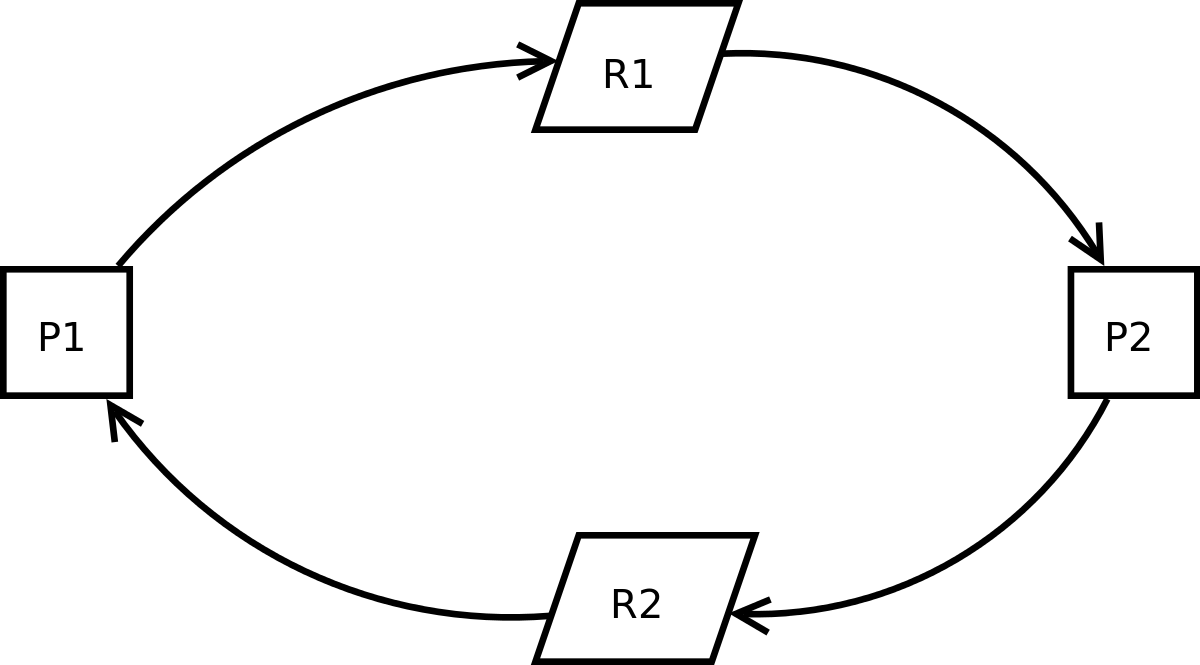
\includegraphics[scale=0.2]{deadlock}
  \centering
  \caption{Exemple d'interblocage}
  \centering
\end{figure}

Souvent pour les programmes avec plusieurs processus et plusieurs ressources, il est difficile de controller l'absence d'interblocages, surtout avec la liberté et puissance offertes par la synchronisation.
D'où l'intérêt de reconnaître ces interblocages automatiquement le plus tôt possible, à savoir, éventuellement, lors de la compilation du programme.

\newpage

\subsection{Problème}

Est-il possible de définir un interblocage pendant l'étape de compilation?

 \subsection{Objectifs}

 Pour répondre à cette question, l'idée est de commencer par créer une version simplifiée d'un langage parallèle en prenant un langage X10 comme un exemple.
 Le compilateur doit reconnaître juste les instructions qu'on a besoin pour créer plusieurs activités parallèles (boucles, conditions, création de nouveaux processus et horloges).\\
 
 Après avoir implémenté un langage qui permet de créer plusieurs activités parallèles avec la synchronisation, il doit être possible de visualiser l'état de toutes les activités au moment d'interblocages.
  on se donne un choix entre simulation d'exécution de programmes parallèles et afficher un message si l'execution se bloquer


\section{La liste des tâches déjà effectuées}

\subsection{Le travail réalisé}
\begin{itemize}
 \item Installation de librairies et IDE pour la langage de programmation \textbf{X10} sur mon ordinateur.\\ Premièrement, il fallait de préparer l'environnement de travail.
 \item Lecture de documentation et plus de documents sur l'interblocage et programmes parallèles.
 \item Exécution de différentes programmes test X10 pour comprendre le problème et voir comment il fonctionne. 
 \item Implementation d'un compilateur inspiré par le langage X10 à l'aide de Lexer et parser (Lex et Yacc).
 \item Génération d'un arbre de la syntaxe abstraite (AST en anglais).
\end{itemize}

\newpage

\section{Le planning prévisionnel des tâches à réaliser}
\begin{description}
  \item[mars] Implementation de simulation d'exécution du programme et captures de traces d'exécution.
  \item[avril] Implementation de visualisation des traces d'execution ou de systèmes mathématique permettant détecter un interblocage.
  \item[mai] Rédiger un rapport avec le bilan de résultats atteins.
\end{description}

\section{Il peut aussi contenir tout ce qui apparaîtra dans votre rapport final. }

\section{Motivation}


 \addcontentsline{toc}{section}{Références}
 \bibliographystyle{alpha}
 \bibliography{../biblio.bib}

\end{document} 

